%%%%%%%%%%%%%%%%%%%%%%%%%%%%%%%%%%%%%%%%%
% Short Sectioned Assignment
% LaTeX Template
% Version 1.0 (5/5/12)
%
% This template has been downloaded from:
% http://www.LaTeXTemplates.com
%
% Original author:
% Frits Wenneker (http://www.howtotex.com)
%
% License:
% CC BY-NC-SA 3.0 (http://creativecommons.org/licenses/by-nc-sa/3.0/)
%
%%%%%%%%%%%%%%%%%%%%%%%%%%%%%%%%%%%%%%%%%

%----------------------------------------------------------------------------------------
%	PACKAGES AND OTHER DOCUMENT CONFIGURATIONS
%----------------------------------------------------------------------------------------

\documentclass[paper=a4, fontsize=11pt]{scrartcl} % A4 paper and 11pt font size

\usepackage[T1]{fontenc} % Use 8-bit encoding that has 256 glyphs
\usepackage{fourier} % Use the Adobe Utopia font for the document - comment this line to return to the LaTeX default
\usepackage{amsmath,amsfonts,amsthm} % Math packages
\usepackage{natbib}

\usepackage[utf8]{inputenc} 
\usepackage[ngerman]{babel}

\usepackage{latexsym}
\usepackage{textcomp}
\usepackage[T1]{fontenc}
\usepackage{bm}% bold math
\usepackage{hyperref}
\usepackage{graphicx}
\usepackage{epsfig}
\usepackage{framed,color}
\usepackage[usenames,dvipsnames]{pstricks}
\usepackage{epsfig}




\usepackage{lipsum} % Used for inserting dummy 'Lorem ipsum' text into the template

\usepackage{sectsty} % Allows customizing section commands
\allsectionsfont{\centering \normalfont\scshape} % Make all sections centered, the default font and small caps

\usepackage{fancyhdr} % Custom headers and footers
\pagestyle{headings} % Makes all pages in the document conform to the custom headers and footers
\fancyhead{} % No page header - if you want one, create it in the same way as the footers below
\fancyfoot[L]{} % Empty left footer
\fancyfoot[C]{} % Empty center footer
\fancyfoot[R]{\thepage} % Page numbering for right footer
\renewcommand{\headrulewidth}{0pt} % Remove header underlines
\renewcommand{\footrulewidth}{0pt} % Remove footer underlines
\setlength{\headheight}{13.6pt} % Customize the height of the header
\usepackage{eso-pic}
\numberwithin{equation}{section} % Number equations within sections (i.e. 1.1, 1.2, 2.1, 2.2 instead of 1, 2, 3, 4)
\numberwithin{figure}{section} % Number figures within sections (i.e. 1.1, 1.2, 2.1, 2.2 instead of 1, 2, 3, 4)
\numberwithin{table}{section} % Number tables within sections (i.e. 1.1, 1.2, 2.1, 2.2 instead of 1, 2, 3, 4)

\setlength\parindent{0pt} % Removes all indentation from paragraphs - comment this line for an assignment with lots of text

%----------------------------------------------------------------------------------------
%	TITLE SECTION
%----------------------------------------------------------------------------------------

\newcommand{\horrule}[1]{\rule{\linewidth}{#1}} % Create horizontal rule command with 1 argument of height

\title{ 
\normalfont \normalsize 
\textsc{Albert-Ludwigs-Universität Freiburg} \\ [25pt] % Your university, school and/or department name(s)
\horrule{0.5pt} \\[0.4cm] % Thin top horizontal rule
\huge Rastertunnelmikroskop \\ % The assignment title
\horrule{2pt} \\[0.5cm] % Thick bottom horizontal rule
}

\author{Friedrich Schüßler und Volker Karle} % Your name

\date{\normalsize\today} % Today's date or a custom date

\begin{document}
\maketitle

\tableofcontents
\begin{figure}[h!]
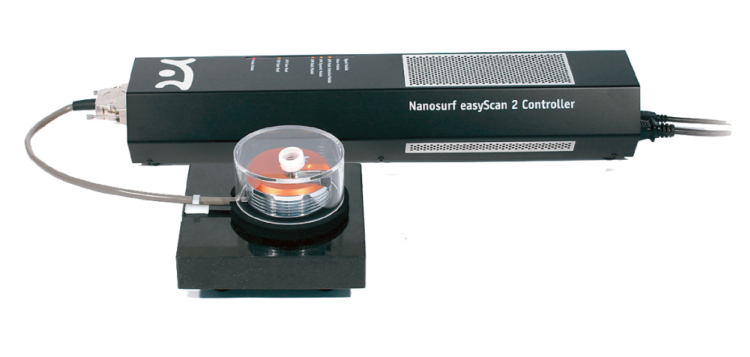
\includegraphics[width=0.75\textwidth]{stm1}

\caption{Easy Scan 2 STM: Rastertunnelmikroskop}
\end{figure}

\thispagestyle{empty}
\newpage
\setcounter{page}{1}


%----------------------------------------------------------------------------------------
%	PROBLEM 1
%----------------------------------------------------------------------------------------

\part{Versuchsprotokoll}
\section{Historische Einführung in die Rastertunnelmikroskopie}
Das Konzept des Tunnelns tauchte in der 
Festkörperphysik auf, als versucht wurde, durch Vakuum bzw. durch
eine Vakuumbarriere zu tunneln \cite{binnig1982tunneling}. Diese
waren zunächst aufgrund der Vibrationen nicht erfolgreich. Nun sind
die Vorteile des Vakuumtunnelns aber evident:
\begin{enumerate}
\item Konzeptuell am einfachsten herzustellende Barriere 
\item Freier Zugang der Elektroden für die Untersuchung anderer
physikalischer und chemischer Prozesse
\end{enumerate}
1981 führten die Autoren G.Binnig, H.Rohrer,
Ch.Gerber und E.Weibel in Zürich zum ersten Mal ein erfolgreiches
Tunnelexperiment mit einem justierbarem Vakuum Spalt durch. 
Ziel war hierbei, das Phänomen des Tunnelns so zu erforschen,
um es in der Spektroskopie und andere Methoden einsetzen zu können. 
Offensichtlich war der schwierige Teil der, die Vibrationen,
die vergangene Experimente fehlschlugen ließen, hinreichend zu
unterdrücken, um somit das eigentliche Signal noch identifizieren zu
können. Dies wurde in dem erwähnten Experiment durch eine 
Dämpfung des Tunnelbauteils mithilfe von Leviation durch
Supraleiter-induzierten Magneten sowie
der Steuerung mit Piezoelementen erreicht. Der Trick liegt darin,
die charakteristischen Frequenzen so zu wählen, dass die 
Eigenfrequenzen des Materials für Vibrationen weit darüber liegen.
Dies ist möglich, indem die Größe des Bauteils sehr klein
skaliert wird, somit können sich keine Vibrationen ausbilden.


\cite{binnig1982surface}
\cite{kittel2013einfuhrung}
\cite{chen1993introduction}

\lipsum[2] % Dummy text

\begin{align} 
\begin{split}
(x+y)^3 	&= (x+y)^2(x+y)\\
&=(x^2+2xy+y^2)(x+y)\\
&=(x^3+2x^2y+xy^2) + (x^2y+2xy^2+y^3)\\
&=x^3+3x^2y+3xy^2+y^3
\end{split}					
\end{align}

Phasellus viverra nulla ut metus varius laoreet. Quisque rutrum. Aenean imperdiet. Etiam ultricies nisi vel augue. Curabitur ullamcorper ultricies

%------------------------------------------------

\subsection{Heading on level 2 (subsection)}

Lorem ipsum dolor sit amet, consectetuer adipiscing elit. 
\begin{align}
A = 
\begin{bmatrix}
A_{11} & A_{21} \\
A_{21} & A_{22}
\end{bmatrix}
\end{align}
Aenean commodo ligula eget dolor. Aenean massa. Cum sociis natoque penatibus et magnis dis parturient montes, nascetur ridiculus mus. Donec quam felis, ultricies nec, pellentesque eu, pretium quis, sem.

%------------------------------------------------

\subsubsection{Heading on level 3 (subsubsection)}

\lipsum[3] % Dummy text

\paragraph{Heading on level 4 (paragraph)}

\lipsum[6] % Dummy text

%----------------------------------------------------------------------------------------
%	PROBLEM 2
%----------------------------------------------------------------------------------------

\section{Lists}

%------------------------------------------------

\subsection{Example of list (3*itemize)}
\begin{itemize}
	\item First item in a list 
		\begin{itemize}
		\item First item in a list 
			\begin{itemize}
			\item First item in a list 
			\item Second item in a list 
			\end{itemize}
		\item Second item in a list 
		\end{itemize}
	\item Second item in a list 
\end{itemize}

%------------------------------------------------

\subsection{Example of list (enumerate)}
\begin{enumerate}
\item First item in a list 
\item Second item in a list 
\item Third item in a list
\end{enumerate}

%----------------------------------------------------------------------------------------


\bibliographystyle{plain}
\bibliography{Protokoll}
\end{document}
